The solver \acrshort{ui} (\cref{fig:sol_vis}) focuses on allowing the user to compare the solutions to Colourful $k$-center problems using different algorithms. We divide the \acrshort{ui} into three columns: configuration, solution visualisation and information. 

%TC:ignore
\begin{figure}[H]
    \centering
    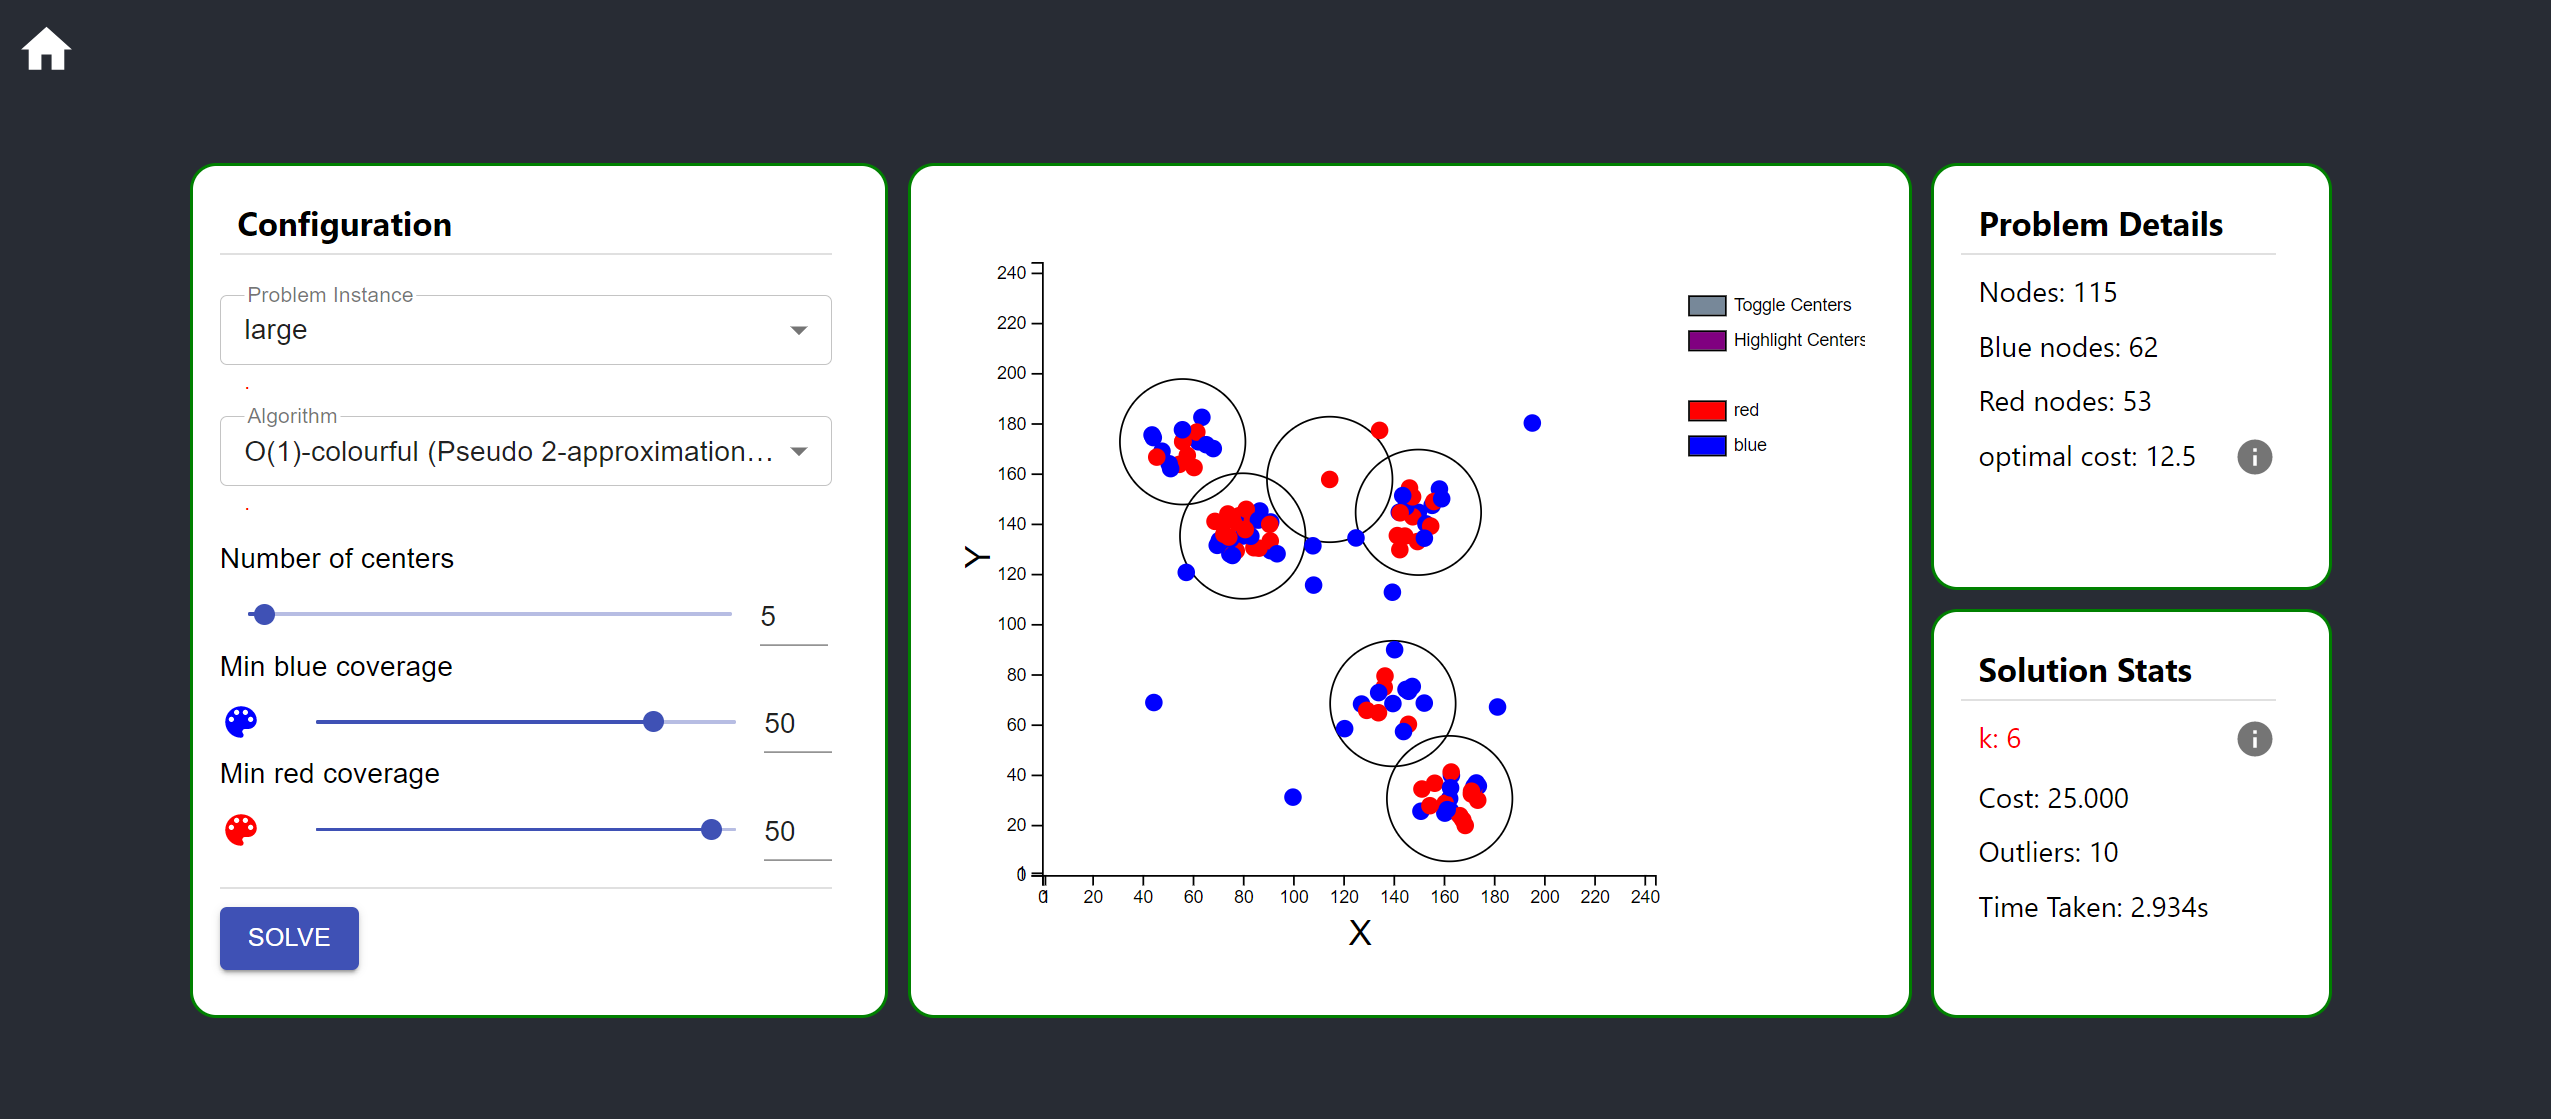
\includegraphics[width=\textwidth]{images/solver_ui/colourful_solve_zoom.png}
    \caption{Solver \acrshort{ui}\\\url{https://colourful-k-center.herokuapp.com/solve}}
    \label{fig:sol_vis}
\end{figure}
%TC:endignore

The configuration column allows the user to choose the problem, algorithm and to adjust the constraints. The visualisation column plots all vertices (colour coded), displaying the coverage generated by a solution. In addition there is an interactive legend which allow users to toggle the displayed data. Finally, the information column displays information about the problem and information about the solution. We use tooltips throughout our \acrshort{ui} to provide additional context.